\problemname{Monopol}
\noindent
Jocke and his friends usually play Monopoly with each other.
After countless games, they have grown tired of the usual rules, so they have changed them a bit.

First, they choose a suitably sized country.
They then look at the road network in the country and choose a sequence of \textbf{different} cities $v_1, v_2, \dots, v_k$ that form a \emph{cycle}.
This means that there is a direct road between cities $v_i$ and $v_{i+1}$ for all $1 \le i < k$ and between $v_k$ and $v_1$, just like on a Monopoly board.
Then they travel to the country and play by driving around the cycle in their cars to buy and sell properties with real money.

However, there is a restriction that makes it difficult to carry out the game: they must find a suitable cycle in the road network.
Some countries have very large road networks.
What makes it even more difficult is that the cycle must have an even number of roads, otherwise, the rules won't work (``Free Parking'' does not end up in the middle, which creates an unbalanced game).

Given all the cities in the country and the roads between pairs of cities, find a cycle consisting of an even number of roads if there is one.

\begin{figure}[!h]
  \centering
  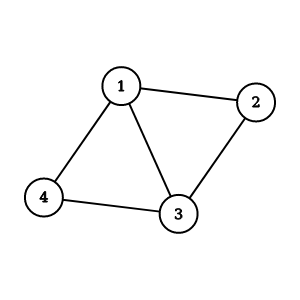
\includegraphics[width=5cm]{sample1.png}
  \quad
  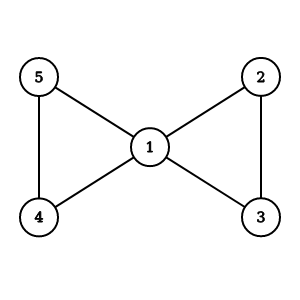
\includegraphics[width=5cm]{sample2.png}
  \quad
  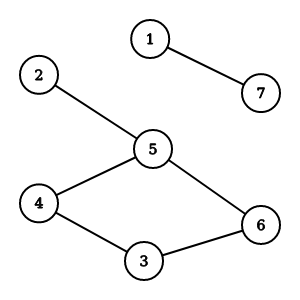
\includegraphics[width=5cm]{sample3.png}
  \caption{Illustration of the countries in the three example cases.}
\end{figure}

\section*{Input}
The first line contains two integers $N$ ($1 \le N \le 10^5$) and $M$ ($0 \le M \le \min(2 \cdot 10^5, \frac{N(N-1)}{2}$), the number of cities and the number of roads in the road network, respectively.

Then follow $M$ lines, each with two integers $a$ and $b$, which means that there is a road between cities $a$ and $b$ in the country ($1 \le a \neq b \le N$).
It is guaranteed that there are no multiple roads between the same pair of cities in the country.

\section*{Output}
If there is no even cycle, print a single line with the string ``\texttt{NO}''.

If there is an even cycle, print a single line with the string ``\texttt{YES}''.
Then, you should print such a cycle.
First, print a line with an \textbf{even} integer $k$ ($4 \le k \le N$), the number of cities in your cycle.
On the next line, print $k$ \textbf{different} integers $v_{1}, v_{2}, \ldots, v_{k}$ ($1 \le v_{i} \le N$) separated by spaces: the cities in your cycle.
It must hold that there are roads between the cities $(v_{1}, v_{2}), (v_{2}, v_{3}), \ldots, (v_{k-1}, v_{k}), (v_{k}, v_{1})$.

If there are multiple possible cycles, you can print any of them.

\section*{Scoring}
Your solution will be tested on a set of test groups, each worth a number of points. Each test group contains
a set of test cases. To get the points for a test group you need to solve all test cases in the test group.

\noindent
\begin{tabular}{| l | l | l |}
  \hline
  \textbf{Group} & \textbf{Points} & \textbf{Constraints} \\ \hline
  $1$ & 18 & $N \le 10$ \\ \hline
  $2$ & 16 & $N \le 100$ and $M \le 200$ \\ \hline
  $3$ & 17 & The cities can be divided into two parts so that no road goes between two cities in the same part. \\ \hline
  $4$ & 13 & All cities in the country have a direct road to at most 2 cities. \\ \hline
  $5$ & 20 & All cities in the country have a direct road to at most 3 cities. \\ \hline
  $6$ & 16 & No additional constraints. \\ \hline
\end{tabular}


